\section[Problem 3]{Problem 3: Newly Inundated Area of Hengzhou with Guarded Model Transfer}
\label{sec:q3}

\subsection{Study Area and Choice of Imagery}

Hengzhou City lies on the Yu River in southern Guangxi. The study area is its GADM~4.1 boundary, $A_{reg}=3440.09$\,km$^2$ (nominal 3440.4\,km$^2$), as the problem asks for the proportion of the whole region; a second, physical denominator is the floodplain zone $\{\mathrm{REM}\le h^*\}$ inside the boundary, 2079.5\,km$^2$.

Rainy-season cloud rules out optics during the event, leaving radar as the observer. Sentinel-1 passes over Hengzhou exist on 27 June, 4 July and 16 July 2026; none falls on 6 July, so 27 June is the pre-flood baseline and 4 July (two days before the reference date) and 16 July (ten days after) serve as flood-time observations (Assumption~3). Products are terrain-corrected VV/VH backscatter in dB on a 10\,m grid at about 20\,m effective resolution; the latest cloud-free optical scene is Sentinel-2 of 31 May 2026.

\subsection{Verification of the Self-Collected Imagery}
\label{sec:q3_verify}

Before any model is applied, the Hengzhou layers have to be geometrically consistent with each other. We test this against a permanent-water reference $\mathcal W^{ref}=\{\mathrm{WC}=80\}\cap\mathrm{OSM}_{water}$, the pixels that both WorldCover and OSM map as water. Two independent sources agree there, so true water must appear dark in SAR. For each date we search the integer shift that maximizes the dark share on this reference,
\begin{equation}
(\Delta r,\Delta c)=\arg\max_{(\Delta r,\Delta c)}\ \frac{1}{|\mathcal W^{ref}|}\sum_{(r,c)\in\mathcal W^{ref}}\mathbb 1\big[VV(r+\Delta r,c+\Delta c)<-15\ \mathrm{dB}\big],
\label{eq:coreg}
\end{equation}
and correct the raster as $VV^{corr}(r,c)=VV(r+\Delta r,c+\Delta c)$.

At the delivered geotransform only 3.4\%, 4.4\% and 4.9\% of the reference water is SAR-dark on the three dates, which open water cannot be. Shifts of 5.4--6.2\,km north--south raise the dark share to 34.6\%, 35.6\% and 37.8\%. The three dates are also displaced against each other by up to 0.8\,km, without which the change guard would compare different ground. Problems 3, 4 and 5 all use the co-registered SAR. The optical scene fails the same test, 2.6\% of the reference water with $\mathrm{NDWI}>0$ at zero shift, at most 4.1\% under any translation, 35\% valid pixels; optics are absent everywhere in Hengzhou ($m_p=0$), the case M6 modality dropout was trained for, and the optical term drops out of $W_0$.

\subsection{Pre-flood Water and the Physics Detector}

A physics water detector $D_d$ on date $d$ uses the split-based Otsu rule \eqref{eq:ashman} on Lee-filtered VV in dB. On calibrated Sentinel-1 the literal rule with 64-pixel sub-blocks accepted land-cover contrasts as bimodal and labeled 52\% of the city as water at $-6.9$\,dB, the same failure as baseline A on the official tiles. We therefore use 128-pixel sub-blocks and accept a sub-block only if its dark class has a mean of at most $-15$\,dB, a physical condition for open water. The pooled thresholds are $-12.23$, $-12.02$ and $-12.80$\,dB for the three dates, from 245, 245 and 272 accepted sub-blocks. Pre-flood water is the union of independent sources (Assumption~4),
\begin{equation}
W_0=D_{0627}\ \cup\ \{\mathrm{WC}=80\}\ \cup\ \mathrm{OSM}_{water},
\label{eq:W0}
\end{equation}
with an area of 292.57\,km$^2$, of which 182.8\,km$^2$ come from the pre-flood SAR.

\subsection{Transfer of the Problem 2 Model}

Model weights do not change: the five fold models M6 of Problem~2 form an ensemble, each with two MC-dropout passes, ten passes per pixel. Checkpoint hashes equal those of Problem~2. What is mapped is the input representation, with the per-tile rank normalization of \eqref{eq:rank_norm} and the Lee filter of \eqref{eq:lee} on $256\times256$ tiles at 10\,m. Whether dB or linear amplitude $10^{VV/20}$ better resembles the GF-3 training input (Assumption~2) is settled by the two-sample Kolmogorov--Smirnov distance between the normalized Hengzhou land pixels and the official non-flood, non-water pixels,
\begin{equation}
T^\star=\arg\min_{T\in\{\mathrm{dB},\,\mathrm{amp}\}}\ \sup_x\Big|\hat F^{HZ}_{T}(x)-\hat F^{off}(x)\Big|,
\label{eq:ks}
\end{equation}
which is 0.106 for dB and 0.241 for amplitude, and dB is used. Refitting the isotonic map and the area-preserving threshold by \eqref{eq:isotonic}--\eqref{eq:tauA} on the pooled calibration predictions of the five members gives $\tau_A=0.557$.

\subsection{Physical Guards and the Final Sets}

A transferred model sees a new sensor, a new polarization (VV instead of HH) and no optics; its raw mask needs physical filtering. Three guards encode what flood water must satisfy. Water cannot stand far above the drainage network, which we measure by the relative elevation above the nearest mapped drainage, a Euclidean variant of the height above nearest drainage~\cite{nobre2011hand}:
\begin{equation}
\mathrm{REM}_p=\max\big(0,\ z^{DEM}_p-z^{DEM}_{n(p)}\big),\qquad n(p)=\arg\min_{q\in\mathcal D}\lVert \boldsymbol x_p-\boldsymbol x_q\rVert,
\label{eq:rem}
\end{equation}
where $\mathcal D$ is the drainage raster (OSM waterways and water polygons plus WorldCover water) and $z^{DEM}$ the Copernicus 30\,m elevation. New water must darken against the pre-flood pass by a margin $\delta$, as in change-detection chains~\cite{twele2016sentinel1}, and patches smaller than a minimum mapping unit of 50 pixels (0.5\,ha, about 12 independent looks at 20\,m resolution) are speckle. The newly inundated set on date $d$ is
\begin{equation}
\begin{split}
F_d=\mathrm{MMU}_{50}\Big(&\{\bar p\ge\tau_A\}\cap\overline{W_0}\cap\{\mathrm{REM}\le h^*\}\\
&\cap\{VV_d-VV_{0627}\le-\delta\}\Big),\qquad h^*=15\ \mathrm{m},\quad \delta=3\ \mathrm{dB},
\end{split}
\label{eq:F_hz}
\end{equation}
receded and flood-time water are
\begin{equation}
R_d=\big(W_0\cap D_{0627}\big)\setminus D_d,\qquad W_{1,d}=F_d\cup\big(W_0\setminus R_d\big).
\label{eq:W1_R}
\end{equation}
By construction $F_d\cap W_0=\emptyset$ and $F_d\subseteq W_{1,d}$. Both were confirmed on the saved rasters with zero violating pixels. A pre-flood water pixel counts as receded only if SAR saw it as water on 27 June and no longer sees it on date $d$. The literal alternative $W_{1,d}=F_d\cup(W_0\cap D_d)$ would also declare receded every mapped channel that SAR never resolves at 20\,m. It raises the receded area on 16 July from 79.44 to 180.09\,km$^2$ and is reported only for comparison. The areas follow \eqref{eq:def_F} and \eqref{eq:net_identity}:
\begin{equation}
A_{new,d}=\sum_{p\in F_d}a_p,\qquad A_{net,d}=A_{new,d}-\sum_{p\in R_d}a_p,\qquad \rho_d=\frac{A_{new,d}}{A_{reg}} .
\label{eq:areas_hz}
\end{equation}

\subsection{Newly Inundated Area, Net Increase and Proportion}

Table~\ref{tab:q3_results} gives the numbers the five questions require.

\begin{table}[!ht]
\centering
\caption{Newly inundated area by pass}
\label{tab:q3_results}
\begin{tabular}{lccccc}
\toprule
Date & $A_{new}$ (km$^2$) & $A_{net}$ (km$^2$) & $\rho$ & Grade & $\pi$ (G / RS / S / ES) \\
\midrule
4 July 2026 & 24.53 & $-54.70$ & 0.713\% & general & 0.74 / 0.25 / 0.010 / 0 \\
16 July 2026 & 26.90 & $-52.53$ & 0.782\% & general & 0.72 / 0.26 / 0.016 / 0 \\
\bottomrule
\end{tabular}
\end{table}

The newly inundated area is 24.53\,km$^2$ on 4 July and 26.90\,km$^2$ on 16 July, i.e. 0.71\% and 0.78\% of the city. All of it lies in the floodplain zone, where the proportion is 1.29\% on 16 July. By the thresholds of Table~\ref{tab:grade_thr} the city-level flood is ``general'' on both dates, with probability 0.72 on 16 July; the relatively-strong probability of 0.26 comes from bootstrap draws of $\theta_1$, whose lower 90\% bound of 0.75\% lies just below $\rho$. On 16 July the new flood covers 13.60\,km$^2$ of former cropland, 9.45\,km$^2$ of tree cover, 1.88\,km$^2$ of built-up land, 1.53\,km$^2$ of grassland and 0.43\,km$^2$ of bare land. The spatial distribution is shown in Fig.~\ref{fig:q3_newflood_map}.

The 27 June pass is the reference: $W_0$ is defined on it and $F$ is empty by construction, which leaves the two rows of Table~\ref{tab:q3_results} as the only comparable observations. Neither row observes the peak. 4 July precedes it, 16 July follows it by ten days, and that gap is exactly the interval in which the flood rose and fell. $A_{new}$ is a lower bound on the peak inundation; what the pair brackets is the receding limb and the residual water, the peak itself falling between the passes.

\begin{figure}[!ht]
  \centering
  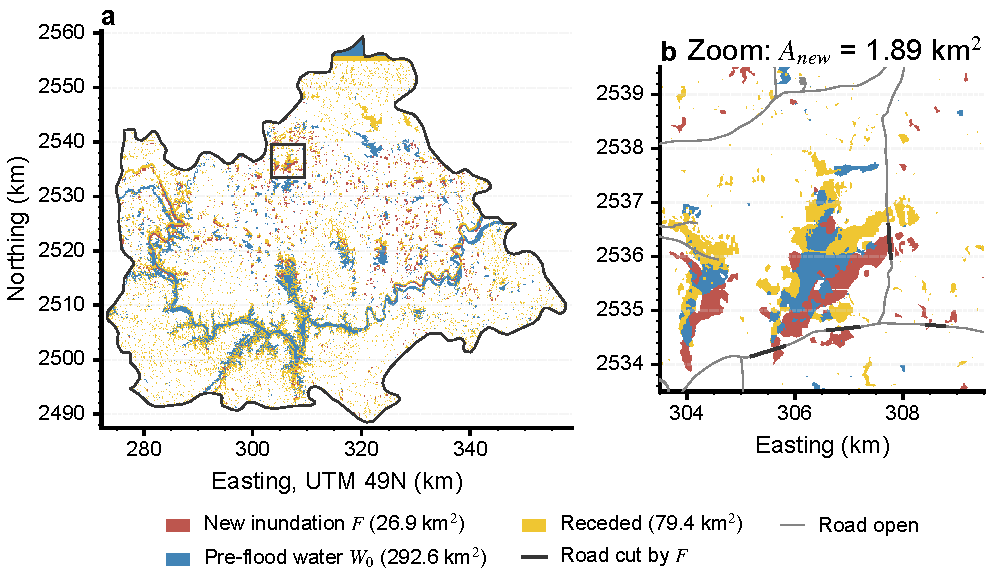
\includegraphics[width=0.90\textwidth,keepaspectratio]{../figures/fig_q3_newflood_map.pdf}
  \caption{Newly inundated area on 16 July 2026}
  \label{fig:q3_newflood_map}
\end{figure}

On 100\,m cells (panel A of Fig.~\ref{fig:q3_newflood_map}) the new inundation follows the Yu River and its tributaries as narrow bands along the valley floors, and the receded water lies on the same corridors. The $6\times6$\,km window with the largest new area is shown at the full 10\,m resolution in panel (B), where flooded fields touch the road network. Those road cuts feed Problem~5. One artifact needs a word: the horizontal band near northing 2555\,km, an edge left by the 27 June co-registration shift where pre-flood SAR is invalid, inflates $W_0$ and $R$ by about 3.4\,km$^2$ each. It carries no new inundation; $A_{new}$, $\rho$ and everything downstream are unaffected, while $A_{net}$ is about 3.4\,km$^2$ too negative.

\begin{figure}[!ht]
  \centering
  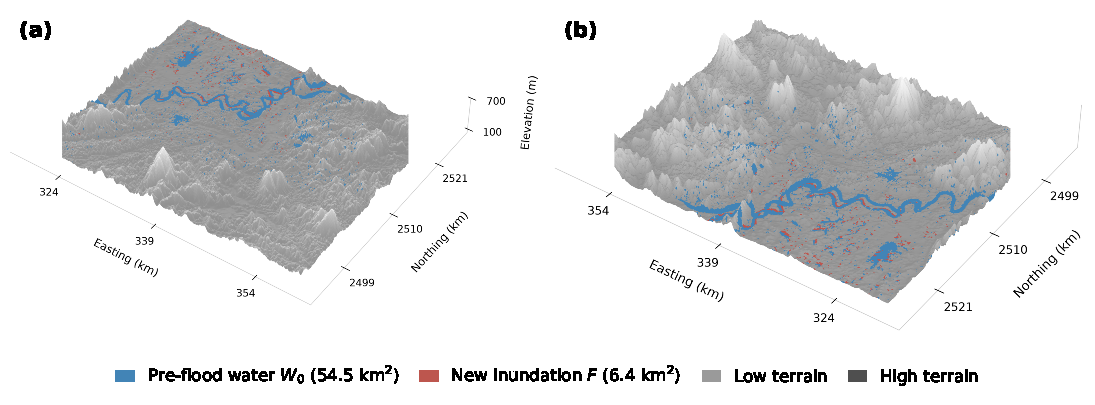
\includegraphics[width=0.90\textwidth,keepaspectratio]{../figures/fig_q3_terrain.pdf}
  \caption{New inundation on the DEM}
  \label{fig:q3_terrain}
\end{figure}

Fig.~\ref{fig:q3_terrain} places those masks on the terrain. The 40$\times$32\,km window is the one with the densest new inundation. It contains 6.4\,km$^2$ of $F$ and 54.5\,km$^2$ of $W_0$, about a quarter and a fifth of the city totals. Every new pixel lies below 200\,m (median 58\,m) and follows the valley floor, whereas the eastern ridge rises to 710\,m and stays dry: the flood is a corridor phenomenon, not a sheet.

Table~\ref{tab:q3_budget} answers why the net increase is negative while new inundation is positive.

\begin{table}[!ht]
\centering
\caption{Guard cascade and water balance (km$^2$)}
\label{tab:q3_budget}
\small
\setlength{\tabcolsep}{3pt}
\renewcommand{\arraystretch}{0.92}
\begin{tabular*}{\textwidth}{@{}l@{\extracolsep{\fill}}rrrr@{\hspace{14pt}}lrr@{}}
\toprule
\multicolumn{5}{c}{Guard cascade} & \multicolumn{3}{c}{Water balance} \\
\cmidrule(lr){1-5}\cmidrule(lr){6-8}
Stage & \multicolumn{2}{c}{4 July} & \multicolumn{2}{c}{16 July} & Term & & \\
\cmidrule(lr){2-3}\cmidrule(lr){4-5}
 & Remaining & Removed & Remaining & Removed & & 4 July & 16 July \\
\midrule
Raw model              & 146.52 & --    & 154.43 & --    & $W_0$             & 292.57 & 292.57 \\
After $W_0$ guard      &  68.43 & 78.09 &  68.85 & 85.58 & Receded $R$       &  79.23 &  79.44 \\
After REM guard        &  44.95 & 23.48 &  44.74 & 24.11 & New $A_{new}$     &  24.53 &  26.90 \\
After $\Delta$VV guard &  34.32 & 10.63 &  36.98 &  7.76 & $W_1$             & 237.87 & 240.03 \\
After MMU              &  24.53 &  9.79 &  26.90 & 10.08 & Net $A_{net}$     & $-54.70$ & $-52.53$ \\
\bottomrule
\end{tabular*}
\end{table}

The balance explains the negative net increase: SAR sees 79.4\,km$^2$ on 27 June that is gone by 16 July, three times the new inundation, 72.4\,km$^2$ of it outside every mapped source (49.4 under tree cover, 16.7 under cropland) and 7.04\,km$^2$ in permanent channels and reservoirs. New water of 26.90 against 79.44 of recession gives $A_{net}=-52.54$ by \eqref{eq:net_identity}, a water-balance quantity rather than the size of the flood; the two flood-time passes agree on the recession to 0.3\% (the literal $-153.19$ comes from the wider 4 July recession). Narrowing the baseline would move the sign: with static water bodies alone (143.4\,km$^2$), the 61.1\,km$^2$ still standing on 16 July would enter $F$ and raise $A_{new}$ from 26.90 to about 88\,km$^2$.

The cascade of \eqref{eq:F_hz} steps from 154.43\,km$^2$ raw to 26.90\,km$^2$ final on 16 July, removing 82.6\% (83.3\% on 4 July), mostly permanent water scored at 0.285 mean probability and excluded by $W_0$. What holds the Hengzhou estimate is the physics guards---drainage, terrain, multi-date change---evidence independent of the network.

\subsection{Transfer Checks and Sensitivity}

Without labels, credibility comes from consistency. The unguarded model mask and the physics change mask $\{\Delta VV\le-3\}\cap D_d\setminus W_0$ overlap at IoU 0.207 with area ratio 2.60: the model sees more candidate water than radar change alone. The VV histogram is bimodal on 16 July (Ashman $D=3.53$) and weakly on 4 July ($D=1.92$); the two new-inundation sets agree at Jaccard 0.391, partial across ten days. The $W_0$ variants order correctly: the union contains the SAR-only $W_0$, so removing it can only shrink $F$, and $A_{new}$ with SAR-only is larger (30.47\,km$^2$). Closing $W_0^{\mathrm{union}}\supseteq W_0^{\mathrm{sar+wc}}\supseteq W_0^{\mathrm{sar}}$ at $26.90<27.29<30.47$\,km$^2$, the 1.4\% step coming from dropped OSM vectors; grade, zone ranking (Spearman 0.996) and the six open depots are identical for both permanent-water variants.

Neither guard parameter $h^*$ nor $\delta$ nor the probability threshold has Hengzhou data to fix it. Fig.~\ref{fig:q3_threshold_surface} recomputes $A_{new}$ over 30 combinations of a threshold shift $\Delta\tau\in\{-0.2,\dots,0.2\}$ and $h^*\in\{5,10,15,20,30,\infty\}$\,m, plus one-at-a-time changes of the other settings.

\begin{figure}[!ht]
  \centering
  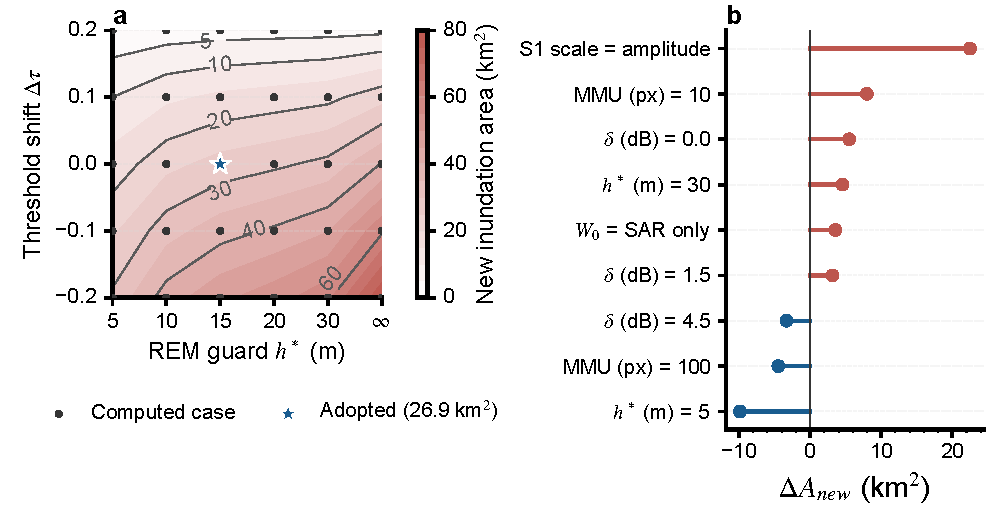
\includegraphics[width=0.90\textwidth,keepaspectratio]{../figures/fig_q3_threshold_surface.pdf}
  \caption{Sensitivity of the Hengzhou new area}
  \label{fig:q3_threshold_surface}
\end{figure}

Panel (A) rises with $h^*$ and falls with $\Delta\tau$, as the guards require: over the grid $A_{new}$ spans 1.57 to 79.52\,km$^2$, and that band travels into every downstream answer. Change margin, water definition, amplitude scale and MMU vary comparably in panel (B) (Table~\ref{tab:sens_chain}). The grade stays ``general'' everywhere, the largest $\rho$ 2.3\% against $\theta_1=5.9\%$: area responds to the guards, the grade does not.

Treating the tile errors of \eqref{eq:conformal} as independent, as in Problem~2, gives $[13.48,40.33]$\,km$^2$ on 16 July, a band that contains the scenario values of the main settings\cite{deepseek2026,qwen2026,doubao2026}.

A target-domain intercept can be priced against physics: new water is dark, low and outside $W_0$ ($\Delta VV\le-6$\,dB, $\mathrm{REM}\le5$\,m, $W_0$ false, 527\,790 pixels), upland bright and high ($\mathrm{REM}\ge30$\,m, $\Delta VV\ge+2$\,dB, 1\,855\,718). The transferred field averages 0.245 and 0.040 on the two anchors, conservative where the physics is certain. Restoring the 22\% prevalence needs $b=+1.19$, which alone moves the raw mask from 154.45 to 415.89\,km$^2$ (2.7$\times$): $\tau_A$ already acts as an intercept, lowering the field so the mask matches the source calibration, and a second intercept read off physics undoes that correction. The two cannot be stacked; we keep $\tau_A$, verifiable on labels, and record $b=+1.19$ as the residual. With 0.285 assigned to permanent water, the flood is recovered from the guards, not from a field deliberately low after two transfers.
